%Kelompok 2
%DONI SAPUTRA(1154030)
%CAHYA KURNIAWAN(1154038)
%IKA SYAM SETIAWATI(1154054)
%SILVY DHARMA FEBRYANA(1154112)
%WIDI DAMAYANTI(1154062)
%ANTARTIKA






\section{Deskripsi Antartika}

\begin{figure}{ht}
\centerline{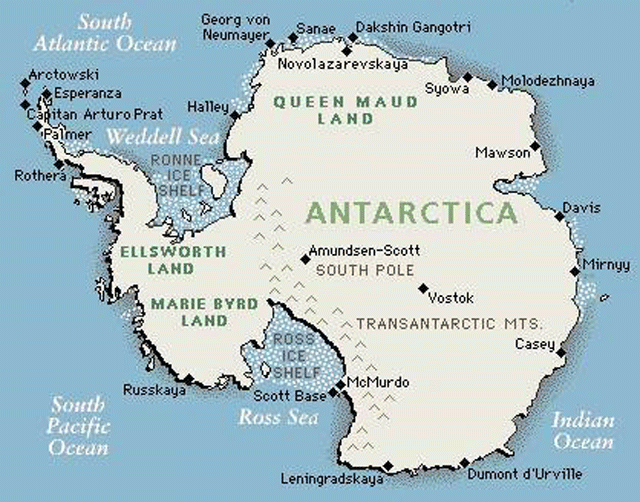
\includegraphics[width=1\textwidth]{figures/antartic.PNG}}
\caption{Peta benua antartika.}
\label{Antartika}
\end{figure}

		Benua antartika adalah suatu wilayah laut perifer yang merupakan sumber informasi utama pada cryosphere cenozoik dan peristiwa 
	kejadian yang mengarah pada perkembangan kurang lebih 36 juta tahun yang lalu. Dilihat dari berbagai data sekarang sudah terlihat bahwasanya 
	garis lintang selatan sudah mengalami perubahan dinamika ekspansi pada lapisan lapisan es nya dan pembusukan melewati akhir Palaeogene dan Neogene. 

	Pada ejarah perubahan iklim disertai dan sangat di pengaruhi oleh lithosphere vertical dan horizontal yang sangat signifikan. Peristiwa perubahan, 
	termasuk evolusi seaways internal utama dan pegunungan\ref{Antartika}. 

		
		Meskipun penyidikan yang dilakukan di tahun pertama pada abad ini antartika kenozoikum penelitian ini adalah bagian dari beberapa kegiatan yang 
	relatif memanjang di sedikit lebih dari 3 dekade di bagian lain dari bumi, kenozoikum rentan terhadap satu penyelidikan, dan dalam sejumlah perkara, 
	hampir 2 abad. Situasi ini sebagian besar dari bagian antartika. Yang sulit adalah penelitian lingkungan, keterbatasan pemanfaatan teknologi canggih, 
	dan realisasi tertunda. Sebagai pentingnya selat lintang selatan yang tinggi untuk isu - isu global, tektonik evolusi seperti  palaeogeography, 
	Palaeo - Oceanography, biogeography, evolusi, dan palaeoclimate biotik. Meskipun komprehensif tinjauan kenozoikum sekarang sudah membuat penampilan yang baru 
	tetapi 25 tahun lalu konozoikum geologi dari antartika hanya mampu melayani beberapa saja.
	
		Terdapat perbedaan yang menarik dalam cara di mana dan kenozoikum Pre - cenozoic studi yang telah dikembangkan di antartika.
	Penelitian dan pendalaman palaeozoic di mesozoikum dan gondwana  geologi yang berfungsi sebagai contoh yang baik. Pada akhir 1950s , 
	ahli geologi banyak dari negara negara berkumpul di antartika dengan cukup detail stratigraphic palaeontological dan informasi dan banyak pengalaman 
	dari banyak tahun penelitian di satu fragmen mantan supercontinent gondwana. Dalam hal kotor, para palaeozoic-mesozoic stratigraphy antartika 
	cermin melaporkan bahwa dari afrika selatan , india , australia , dan amerika selatan. Antartika palaeozoic-mesozoic disebut ilmu pengetahuan untuk 
	memberikan untuk mengukur daerah , stratigraphy , koleksi fosil , analisis dan batuan beku sedimen batu dan daerah analisis .Kebanyakan gondwanas  
	para ilmuwan itu lalu , pengujian dan memperluas pengetahuan dasar yang itu , dalam banyak hal , dikembangkan di beberapa benua. 
	Fosil yang dikumpulkan di Antartika selama 30 tahun telah di dokumentasikan dengan baik di wilayah - wilayah lain Gondwana dan penemuan mereka di Antartika 
	telah sering agak tepat memperkirakan. 
	
		Misalnya, dalam sebuah Pra-Geofisik Internasional kaji ulang tahun, Fairbridge geologi Antartik (1952, mukasurat 88) dicatatkan, 
	"Maukah membingungkan dari semua adalah ketiadaan bukti seretnya proses di gunung batu zaman Permian, yang merupakan kali mengalami Glaciation 
	kuat dalam semua bagian lain di Selatan Hemi ; mengapa sphere Antartika, dari segala tempat akan dikecualikan. Dalam satu dekade laporan-laporan 
	sebagai kemudian hilang tillites dibuat dari Rambu Supergroup dari Trans- Gunung dan lain-lain tempat Antartika. Elemen penting dalam kemajuan yang 
	dibuat oleh Palaeozoic cepat dan para peneliti Mesozoikum adalah mendukung pro- vided oleh IUGS Sub-Commission untuk Gondwana Stratigraphy serta 
	palaeontologi. Para peneliti Cenozoic Antartik tidak memiliki dukungan dari sebuah organisasi payung, walaupun IUGS Kuartenari Internasional Association 
	mungkin telah memainkan peran lebih aktif, terutama di daerah seretnya proses dan proses interglacial Antartika. Studi Cenozoic Antartik kekurangan, 
	antara lain, sebuah elemen prediktif, dan banyak kemajuan yang telah serendipitous, selalu mengherankan, dan sering kontroversial. 
	Antartika, geografis belaka pencerahan telah, untuk tiga dekade terakhir, dijamin tingkat geografis, dan isolasi intelektual untuk pekerja Cenozoic 
	dari banyak negara. Sementara ada sebuah koleksi tingkat kuat dan dokumentasi, hanya ada sedikit koordinasi dan jangka panjang perencanaan di antara 
	berbagai perusahaan nasional. Dalam jumlah relatif kecil melimpahnya sinar Cenozoic di Antartika sekarang dengan cukup lancar didokumentasikan dan 

	sedikit yang dapat diperoleh didaur ulang usaha sebelumnya hanya untuk penguatan marjinal. Kita harus berkonsentrasi pada cara-cara untuk kausingkapkan 
	98\% dari geologi Cenozoic kita masih belum menemukan! Lebih penting lagi, kita harus melihat `austral' Cenozoic di lebih ketentuan global\cite{peter1990Antartica}.
	

\subsection{Antartika dan Cenozoic cryosphere}

		Jika seseorang untuk satu dari satu fenomena geologis yang disajikan untuk menyorot pentingnya Cenozoic Antartika ia harus realisasi yang tinggi 
	selatan latitude Cenozoic perubahan iklim goyangan) yang dicetuskan dampak yang signifikan yang jauh melampaui batas benua untuk sekurang-kurangnya 
	dua pertiga dari waktu Cenozoic. Setelah Ia mengatakan semuanya itu, satu juga harus mengamati bahwa penelitian Cenozoic Antartika dan global 
	masyarakat telah, hingga sangat baru-baru ini, bekerja secara mandiri dan terlepas dari satu sama lain dan telah ada unawareness umum oleh mantan 
	kelompok yang berkembang pesat Cenozoic Antartik alas data dan kompleksitas seretnya proses-proses deglacial. Untuk banyak palaeo-ahli lautan, 
	ia telah atribut yang cukup untuk `dingin' tren data proxy mereka untuk `cryogenic' kejadian ke selatan, barangkali glaciation di Antartika. 
	Dalam beberapa tahun terakhir telah melihat sebuah sambutan pindah ke arah yang lebih besar di tingkat interaksi antara kedua masyarakat. 
	Namun, masih lebih banyak dan integratif dasar research untuk dapat dicapai dalam dan antara wilayah dan alas data kelautan.
	
	
\subsection{Peran dari laut dalam Proyek pengeboran dan laut Program Pengeboran}
		
		memiliki banyak untuk mengubah studi Cenozoic global dari sebagian besar aktivitas berbasis tanah untuk satu spanning hampir di seluruh bumi. 
	High latitude pengeboran usaha-usaha kaki 28 (selatan-timur Laut Ocean-Ross OceanSouthem India di tahun 1973), 35 (selatan-timur Samudera Pasifik di 1974), 
	113 (Laut Weddell- Samudera Atlantik Selatan pada tahun 1987), 114 (subantarctic Samudera Atlantik Selatan pada tahun 1987, 
	119 (Prydz Bay-Southern Samudera India pada tahun 1988) dan 120 (dataran tinggi Kerguelen-selatan-timur Samudera India pada tahun 1988) telah dilakukan 
	banyak untuk membawa bersama-geologi Cenozoic dari Antartika dan subantarctic yang tepat dan ketika latitud temperate (Gbr. 1). 
	Sementara banyak rincian empat kaki Antartik masih menunggu, kapal penyelidikan berbasis Antartika, bersama-sama dengan penelitian pada benua itu 
	sendiri, telah memperkuat pemahaman kita tentang kedua-dua dahulu kala dan sejauh mana Cenozoic glaciation di belahan bumi selatan.
	

\subsection{evolusi Cenozoic Palaeoenvironments di Selatan}

		Pada tahun 1986, Sidang Internasional Perserikatan Ilmiah (ICSU) Komite Ilmiah pada Antarctic Research (mengenai pelipis) didirikan grup dari 
	kalangan dokter spesialis pada evolusi Cenozoic Palaeoenvironments di Selatan ketika latitude tinggi. Perintah kepada kelompok internasional ini 
	disertakan: korelasi dan integrasi Antartika dan Cenozoic palaeoen viron mentale ecords laut dengan orang-orang di selatan ketika latitud 
	tinggi, dan pengakuan dan evaluasi gfobal Cenozoic penting, palaeu tektonik mengadakan dan peristiwa palaeoclimatic-disimpulkan dari penelitian 
	geologi Antartika. Dalam tiga tahun terakhir dalam grup bekas luka dari kalangan dokter spesialis telah berpartisipasi dalam beberapa dinner symposia 
	dan telah menyetel tentang mengkaji topik Cenozoic penting di lokakarya khusus. Misalnya, pada akhir 1988 Grup dari kalangan dokter spesialis 
	mensponsori `Lokakarya Pengeboran Kutub' dalam kerjasama dengan Yayasan Sains Nasional AS; dan pada awal 1989 mengadakan pertemuan pada geochronology 
	Cenozoic Antartika. Pertemuan masa depan dan ini berfokus pada topik-topik yang dianggap penting, terutama dalam memahami peran global 
	geologi Cenozoic Antartik.
	
	
\subsection{Program Geosphere-Biosphere Internasional}


		Dengan penyebaran ICSU `Geosphere Internasional- Program Biosfir'(IGBP),p olar para peneliti Cenozoic dihadirkan dengan beragam peluang baru. 

	Baru-baru ini bekas luka mengakui peran utama dalam wilayah kutub selatan harus memainkan di masa depan oleh penerbitan 'Peran Antartika dalam 
	Perubahan Global' (ICSU Tekan). Inisiatif IGBP yang prihatin prinsipnya dengan (p. 7), 'interaksi kunci dan perubahan yang signifikan pada waktu 
	timbangan dekade untuk berabad-abad...."; namun, pada mukasurat 23 dinyatakan, 'Antartika berpendapat rekod ekstensif iklim masa lalu dan perubahan lingkungan. 
	Inti es dan core laut dapat menumpahkan lampu baru seperti pada perubahan. Dari permukaan particularpromisea rekecore batu.
	
	
\subsection{Wilayah penting dan daerah yang dikenali sejak tahun Geofisik Internasional (1957-1708)}

		Tahap sekarang penyelidikan bermula pada 1957 selama Tahun Geofisik Internasional. Selama penyelidikan selama 30 tahun beberapa wilayah kunci 
	muncul sebagai penting, terutama. Ini adalah: Seymour Island, dengan terkena Cretaceous-Palaeocene penting- Eocene successions, dan remarkablef 
	fosil fauna dan flora: Raja George Island, dengan Eocene-Oligocene penting-Miocene successions lebih rendah dari fossiliferous sedimen glacigene 
	laut dan interbeded dapat ditarik volcanics: dan selatan- Ross Barat Laut (Victoria Tanah Basin dan bokor lainnya) dan berdekatan dengan wilayah 
	Gunung Transantarctic, dengan Oligocene-MiocenePliocene-Pleistocene glacigene penting di diantaranya- cessions (Gbr. 1). 
	Baru-baru ini, Amery graben-Wilkesfpensacola Prydz Bay dan bokor-bokor penyiraman juga telah menjadi wilayah penting untuk Palaeogene dan studi Neogene. 
	Mayoritas Cenozoic Antartik literatur selama tiga dekade terakhir berasal dari lapangan dan penyelidikan laboratorium di wilayah dipisahkan secara luas ini.
	Sementara Cenozoic outcrops di wilayah-wilayah ini berisi floras macrofaunasa yang sangat baik ke-52, dan telah dikaitkan dalam beberapa contoh dengan 
	dapat ditarikhkan bahan gunung berapi, hanya rovide successionsp temporal kesinambungan sporadis. Hiatuses adalah biasa dan banyak-kurang bergandengan usia. 
	Sementara kutub dan extra-palaeo kutub menggandakan dan peristiwa iklim telah di dokumentasi kan dalam negeri-basedexposures ini, 
	ia juga jelas bahwa stratigraphicalr ecord tidak memadai untuk spektrum luas Cenozoic studi geologi.
	
	
\subsection{Pengeboran ilmiah (1972-1954)}

		Sejak tahun 1972, serangkaian pengeboran ilmiah ventures telah sangat memperbaiki geografis, dan jangkauan temporal untuk kedua-dua Palaeogene 
	dan Neogene (buah ara 1,2,3). 70 lubang simulasi selesai dalam 18 tahun terakhir jatuh ke dalam dua kategori utama. 3 1 situs-situs menaruhnya di darat 
	atau dari laut dekat pantai-platform es, dengan total penetrasi 3793 m (12 444 kaki), dan 39 kapal laut dalam simulasi berbasis lubang-lubang.
	
	diperhatikan di bawah bahwa latitudepalaeogene tinggi selatan dan rekaman Neogene kompleks interelated frekuensi tinggi mengadakan geologis, 
	peristiwa iklim dan, banyak di antaranya yang hanya dapat diatasi jika sampling adalah pada 25 untuk 50 000 tingkat tahun. Sedikit kemajuan akan dibuat 
	dalam palaeoenviron- dan studi palaeoclimatological mental tanpa peningkatan yang signifikan dalam penggunaan teknologi pengeboran yang paling maju 
	di kedua Antartika dan di wilayah subantarctic.
	

\subsection{Pelat dan interaksi microplate}

		Pelat dan interaksi microplate disintegrasi Gondwana dalam Mesozoic dan Cenozoic, menjadi kecil continental pelat dan microplates, disediakan rumit 
	dan pernah mengubah konfigurasi dari tanah dan wilayah laut di bagian selatan ketika latitud tinggi. Pemisahan Australia dan Antartika dalam Eocene, 
	pemisahan di selatan Amerika Selatan semenanjung dari Antartika dekat batas Oligocene-Miocene, subsequentd pembangunan sirkulasi laut sekitar 
	Antartika, dan efek yang dihasilkan pada perubahan iklim dan biogeography telah didokumentasikan dengan baik dalam literatur (lihat Kennet 1982 untuk 
	ringkasan pandangan dan lengkap dari literatur justu berlawanan). Sementara Cenozoic episode tektonik di pinggiran benua tersebut adalah dengan cukup 
	lancar didokumentasikan, orang-orang dalam wilayah pedalaman tidak. Setelah kedua adalah dimengerti dengan baik kita akan lebih mampu untuk menilai 
	pewaktuan dan perute-an jalur sirkulasi laut ke dan di Antartika (Gbr. 4). Tidak jelas, misalnya, apakah yang dicurigai dan masa kelam erosional tektonik 
	yang disediakan dalam peredaran air merutekan sekitar dan melalui bagian Antartika di berbagai waktu selama Cenozoic, dan apakah saluran ini disediakan 
	sebuah link efektif antara berbagai sektor Atlantik selatan, Pasifik dan lautan India. Studi masa depan harus menekankan pembatasan, dan interaksi antara, 
	pelat dan microplates, bersama dengan penentuan masa gerakan vertikal dan horizontal.
	
	
	
	

	
		
	
	
		
